\chapter{SELECTするってどんなこと}

\section{SELECTとはなにか}

リレーショナルデータベースへの問い合わせに使う、SELECTとななんなのでしょうか。
SELECTを一言でいうと、フィルタです。
つまり、検索対象となるテーブルから実行結果のテーブルへの写像関係である、ということもできます。
それを理解するために、SELECTとはどのような作用をしているか、順を追ってみていくことにしましょう。

\subsection{SELECTによる検索}

SELECTは、あるテーブルに属する全てのレコードから、条件に一致するレコードを選びます。
そして、対象となるテーブルから選択されるレコードがいくつあっても、その全てに合致する条件を一度書くだけです。
このとき、手続き型言語のように、ループを書く必要はありません。

つまり、対象とすべき要素全てに該当する条件を書けばいいというのが、SELECTの特徴です。ですが、手続き型言語になれていると、レコードの1件ずつに対してマッチングを行わないことに、不安を感じるかもしれません。

grepというテキストの検索ツールを使ったことがあるなら、検索したい部分の条件を一度書いたら、対象となるテキストファイルの全ての行に対して、その検索が適用されます。
そして、テキスト全体に対して結果が得られるというのを疑問に思わないでしょう。

では、テキストファイルがテーブルであり、テキストファイルの行がレコードであると考えてみたらどうでしょうか。
テキストファイルというテーブルに対してSEKLECTを実行すれば、検索条件に該当する、すべての行というレコードが得られます。
実際、MySQLには、テキストファイルであるCSVをそのまま、検索対象のテーブルとすることができるエンジンがあります。

このように、SELECTには、テーブルの全てのレコードを対象に実行される、という性質があります。

\subsection{SELECTの実行結果}

SELECT文の実行結果は、テーブルです。そのアトリビュートは、SELECT文のなかで設定されたものになります。
このとき、結果となるテーブルをつくるとき、レコードのアトリビュートの名前や型を変更したり、その値を加工することもできます。

また、SELECTの実行結果であるテーブルには、名前がありません。
そして、寿命は、SELECTが実行されたときだけとなります。
そのため、この結果を保存するためには、SELECTの結果をレコードとしてもつテーブルをCREATEするか、外部プロセスで、リレーショナルデータベースの外に取り出す課する必要があります。

\subsection{SELECTと結果の加工}

SELECTでは、結果を加工することができます。例えば、以下のようなSELECT文を考えてみましょう。xaxisというテーブルのレコードは、zというアトリビュートを持ち、数値が入っているとします。

\begin{verbatim}
SELECT x+1 as y FROM xaxis;
\end{verbatim}

このSELECT文は、xaxisテーブルの全てのレコードを対象としています。xaxisテーブルのレコードがもつ、xというアトリビュートの値に1を足したアトリビュートyをもつレコードをつくり、そのレコードからなる名無しのテーブルをつくるという動作をします。
このように、SELECTは、元のテーブルに影響を与えず、加工されたレコードからなる結果のテーブルを作る、という動作します。

\subsection{SELECTの対象となったテーブル}

あるテーブルに対してSELECTを実行したとき、その対象となったテーブルは全く変化しません。
これは、とても重要な性質です。

SELECTの対象となるテーブルとはSELECTへの入力である、そう考えてみましょう。
このとき、入力側はSELECT分の実行によって変化しません。
このことを、SELECTには入力側への副作用が無い、というような言い方をします。

また、実行結果のテーブルをつくるとき、そのアトリビュートの名前や型を変更したり、値を加工したりできる、という書方をしました。
その場合でも、対象となった側のテーブルへの副作用はありません。

\subsection{SELECTと日付関数}

SQLには、現在時刻を得るための関数があります。
これは、タイムスタンプを記録するために用いるもので、MySQLやPostgreSQLでは、now()という名前です。

\begin{verbatim}
SELECT now();
\end{verbatim}

このようなSELECT文を実行したら、以下のように結果がテーブルで返されます。

\begin{verbatim}
+---------------------+
| NOW()               |
+---------------------+
| 2019-04-11  01:23:45| 
+---------------------+
\end{verbatim}

jこれは、仮想的な全時刻のテーブルから、SELECT文の実行時間を関数now()で取り出したとかんがえることができます。
結果は名前のないテーブルであり、now()という名前のタイムスタンプのアトリビュートをもちます。
そして、その名前のないテーブルは、SELECT実行の日時をもつレコードを一つだけ持っています。

\subsection{SELECTというフィルタ}

\begin{figure}[htbp]
	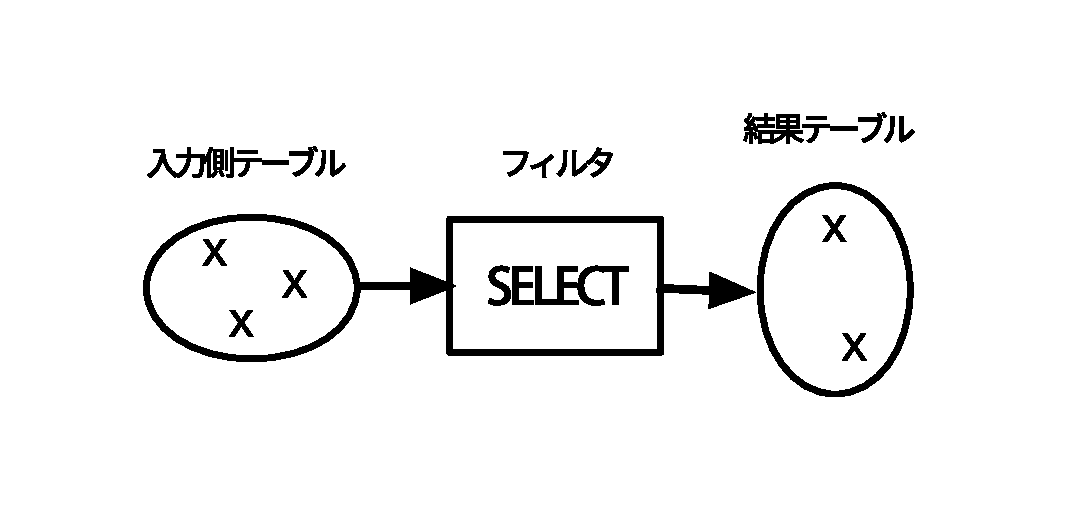
\includegraphics[width=12cm,clip]{draw/filter.eps}
	\caption{フィルタとしてのSELECT}
	\label{fig:filter}
\end{figure}

SELECTがなにをするものかを一言であらわすなら、それは、テーブルを対象としたフィルタであるということです。
ここまでで挙げた、SELECTの性質を振り返ってみましょう。

\begin{itemize}
  \item テーブルを対象とする
  \item 取り出したいレコード全てにマッチングする条件を設定する
  \item 実行結果としてテーブルが得られる
  \item 実行結果のテーブルを作るとき、アトリビュートの型や名前の変更、値の加工ができる
  \item 結果のテーブルの寿命はSELECTが実行されたときだけ
  \item 検索対象となったテーブルへの副作用が無い
\end{itemize}

このような挙動をするなにかを説明する言葉は、フィルタです。
フィルタという言葉を使うと、テキストフィルタとの類推を考えるかもしれません。
代表的なテキストフィルタ言語としてawkがあります。
テーブルをテキストファイル、レコードをテキストの行と考えたとき、SQLのSELECTとawkは、似たようなkとをしています。

つまり、フィルタの本質とは、入力となる集合から結果である集合への変換規則です。











\section{SELECTと関数}

SELECTがフィルタであるということを、数学の用語を使ってあらわせば、SELECTは写像関係である、と言う表現になります。

ここで、テーブルという言葉を、集合にもどしてみましょう。このとき、SELECTは、ある集合から別の集合への、要素の対応関係を表している、とウッ言い方をすることができます。
つまり、SELECTの結果がテーブルであると言うことは、SELECTは集合間の写像関係を表しているということができます。

集合間の写像関係とは、すなわち関数です。つまり、SELECT文とは、数学の言葉で表現すれば、関数であると考えることができます。

\subsection{数学の関数をSELECTであらわす}

$y=x+1$という初等関数を考えてみましょう。SELECTが写像であり、関数であるなら、この関数をSELECT文で欠けるはずです。
ここで、$x$として取りうる値の全てがレコードとして納められているテーブル、xaxisを仮定します。

\begin{verbatim}
SELECT x+1 as y FROM xaxis;
\end{verbatim}

ここでは、ごく簡単な例で説明をしましたが、より複雑な関数をSELECTで書くこともできます。

もし、xaxisというテーブルのレコードで、全ての実数を網羅していれば、このSELECT文とその結果は、$y=x+1$という関数と全く同じものとなります。
ただし、実際のSQLは、要素数が有限なテーブルをもちいます。そのため、テーブルxaxisのレコードは、$x$として入力したい値の集合であり、結果のテーブルは、xのレコードとして存在する値に対応する、yの値をレコードとしてもつテーブルになります。

\begin{figure}[htbp]
	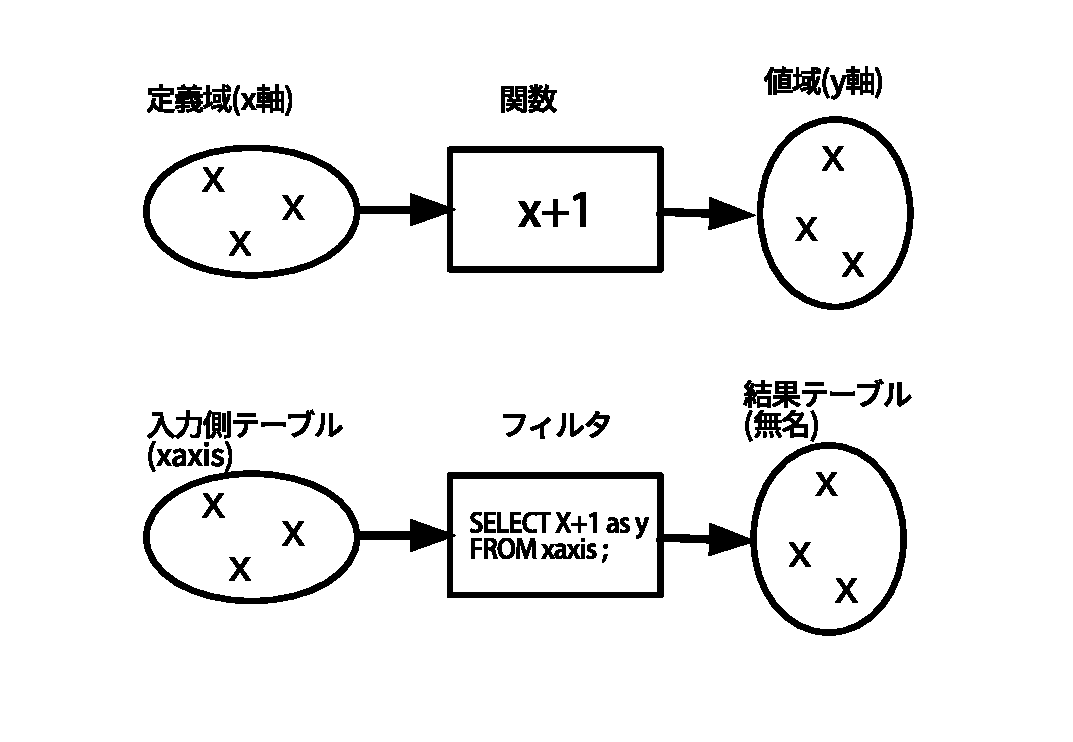
\includegraphics[width=12cm,clip]{draw/function.eps}
	\caption{関数とSELECT}
	\label{fig:function}
\end{figure}

また、ここまで何度も説明したとおり、SELECTは入力に対して副作用を持ちません。
数学の言葉を使えば、入力に対して直交であるという言い方もできます。
つまり、入力と出力の関係を、直交座標系であらわすことができます。
以下のようなSELECT文の結果のテーブルのレコードを、アトリビュートを使った直交座標系における場所に置けば、それは、$y=x+1$のグラフに他なりません。

ただし、実際のテーブルのレコード数は有限です。そのため、拡大すれば必ず、直交座標においたレコードとレコードの間にはすきまがあります。

\begin{verbatim}
SELECT x,x+1 as y FROM xaxis;
\end{verbatim}

\begin{figure}[htbp]
	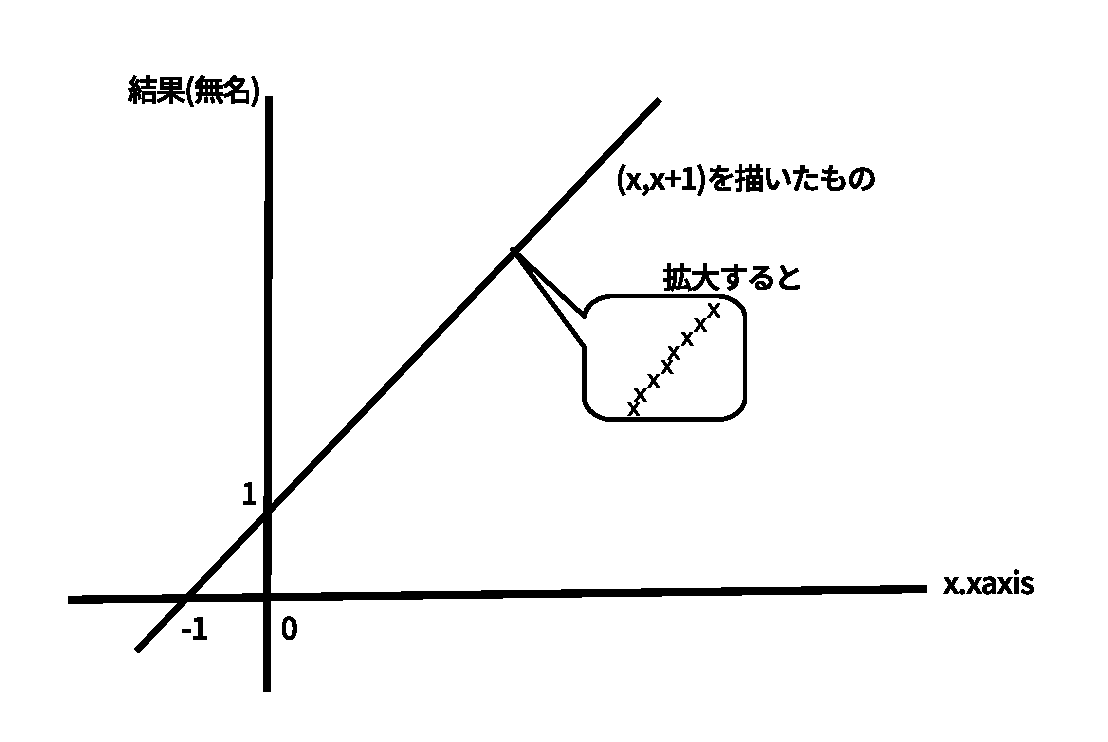
\includegraphics[width=12cm,clip]{draw/plot.eps}
	\caption{結果テーブルと直交座標系}
	\label{fig:function}
\end{figure}

\subsection{SELECTと結果の等価性}

ある入力に対して、SELECTは関数として作用します。
では、結果のテーブルとSELECTの関係は何でしょうか。

入力となるテーブルと、そのレコードが同じであれば、SELECTの結果であるテーブルは、常に同じアトリビュートを持ち、そこに含まれるレコードも同じものになります。
つまり、入力側が常に同じであるとき、関数であるSELECT文と、結果のテーブルは等価、と考えることができます。
SELECT文が分かっていれば結果のテーブルは一意に決まります。
また、入力されるテーブルと、結果のテーブルが判明していれば、関数であるSELECTをつくることができます。

全ての結果の集合と、関数は等価である、と、考えると、SELECT文とその結果のテーブルは等価である、と考えることができます。
また、SELECTを命だ論理の命題と見なせば、ある命題に関して、命題と、その全ての解を網羅した集合は等価である、という表現をすることがあります。

\subsection{なぜサブクエリを使えるのか}

\begin{figure}[htbp]
	
\includegraphics[width=12cm,clip]{draw/subquery.eps}
	\caption{サブクエリ}
	\label{fig:subquery}
\end{figure}

SQLでは、テーブルの名前を書くべきとろこに、SELECT文を書く、サブクエリを使うことができます。本来は、テーブル名を書くところで、SELECT文を書くことができるという機能です。
この機能の根拠は、SELECT文と結果のテーブルは等価であるという性質になります。

サブクエリでは、そのSELECT文の結果がレコードであるテーブルを使ったと見なして、文を実行します。
つまり、クエリの中で、サブクエリのSELECT文が、テーブルのようなものとして扱われているということです。

リレーショナルデータベースで、集合とはテーブルのことです。そのため、SELECT文によるサブクエリと、その結果がレコードであるテーブルは、等価であるということになります。これが、SQLでサブクエリを使うことができる根拠です。

また、SELECTの結果となるテーブルに名前が無いことは、これまで説明たとおりです。
つまり、サブクエリは一種のラムダ式と考えることもできます。
ですが、SQLは関数型言語にはなり得ません。それについては、この次に説明をします。

\section{SQLと関数型言語}

ここまでで、SELECTはフィルタであり、フィルタはもとの集合に対する関数であり、命題であるという解説をしました。そうなると、SELECTは題意球関数であるのかが気になります。結論から行くと、SELECTは題意球関数ではありません。そのため、SQLは、関数型言語ではありません。

本性の最後に、その理由を説明しましょう。

\subsection{SELECTと第一級関数・第一級オブジェクト}

第一級関数とは、引数や戻り値として、関数を扱うことができる言語です。あるSELECT文という関数への入力とはテーブルです。
このとき、テーブルの代わりにサブクエリを使うことができるので、入力に関数を取ると考えることができます。
ですが、この入力は引数ではないため、サブクエリを使っても関数を引数としたことには鳴りません。

また、SELECT文は、その出力に実行可能な形で、SELECT文という関数を返すことができません。SELECTから出てくるのは、結果の集合であり、値しか出すことができないと考えることができます。

これらの理由から、SELECTは第一級関数ではありません。
つまり、関数を含む全ての様子を無制限に取り扱える、第一級オブジェクトではありません。

\subsection{SQLは関数型言語なのか}

SELECTとは関数であり命題である、この章で繰り返し説明したテーマです。では、SQLは関数型言語なのでしょうか。
その答えは、SQLは、関数型言語の定義から外れるため、ノーとなります。

SELECTは戻り値として関数、つまりSQLの中で実行可能な形でSELECT文をはじめとするSQL文を生成することはできません。
これは、SQLが、入力と出力に制限を付けない、第一級オブジェクトではないということでもあります。
関数型言語の用件として、第一級オブジェクトを扱えること、というものがあります。そのため、SQLの構文は第一級関数ではなく、第一級オブジェクトでも無いため、SQLは関数型言語ではありません。
